\section{Présentation du projet}

\subsection{Annoncé}
\enquote{Étant donné un échiquier de dimension $m \times n$, énumérer tous les circuits hamiltoniens réalisés en utilisant uniquement les mouvements du cavalier dans le jeu d'échecs. Même question, mais en énumérant le nombre de chemins hamiltoniens "ouverts" (origine et destination différentes).}

\subsection{Travail à réaliser}
Le but premier est de réaliser une application pouvant calculer le nombre de circuits et de chemins hamiltoniens différents que peut emprunter un cavalier sur un échiquier de dimension choisie par l'utilisateur.

Ceci s'apparente donc à un parcours de graphe, chaque case de l'échiquier est un sommet et chaque mouvement possible à partir de cette case vers une autre est une arête du graphe.

\begin{figure}[h]
\begin{center}
   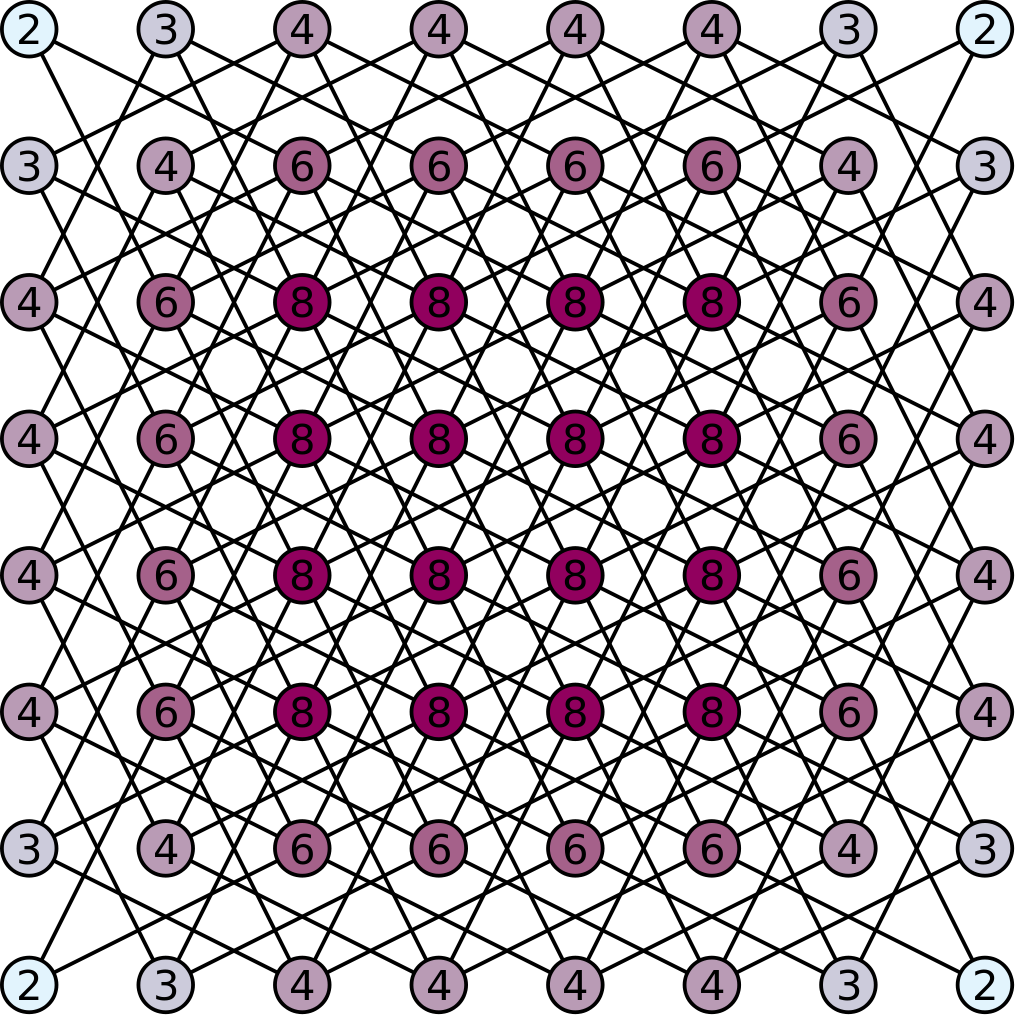
\includegraphics[scale=0.25]{img/graph_cavalier.png} 
   \caption{\label{cavalier_graphe} Graphe du cavalier sur un échiquier $8 \times 8$(inclure source ici wiki)}
   \end{center}
\end{figure}

Le graphe de la figure ~\ref{cavalier_graphe} représente les déplacements possibles pour un cavalier sur un échiquier classique. Le degré de chaque nœud y est précisé. 

La réalisation de ce travail implique la génération d'un graphe similaire, généralisé à n'importe quelle taille $m \times n$. Ainsi que le calcul de tous les chemins/circuits hamiltoniens possibles sur le graphe généré. 

Néanmoins d'autres fonctionnalités peuvent êtres intéressantes pour l'utilisateur, comme par example afficher un chemin hamiltonien généré. Elles seront ajoutés lors du développement.

